% $Id: solution.tex 
% !TEX root = ../main.tex

\section{Flik: A Bugs Life Debugger}
\label{sec:solution}

The black box behavior of \ac{ML} and \ac{RL} agents posit a problem to understand agents and 
their behavior, specially if unexpected behavior is observed. We posit debuggers as an appropriate 
tool to understand agents' behavior. Moreover, we posit debuggers with the possibility to modify 
programs' state and continue execution using new execution paths are even more appropriate and 
suitable to understand \ac{RL} agents, given their intrinsic nature of continuous interaction with the 
environment. However, currently, there is no debugger for \ac{RL} programs with the desired 
features. The reason for this is that most of the debuggers are postmortem, or do not allow developers
to go back in time to replay and analyze the program state. Additionally, most of the debuggers do not 
allow developers to modify variables. In order to contribute to the development of \ac{RL} programs, 
debugging tools should exhibit the following features:

\begin{description}
    \item[Stepping back:] Due to the execution loop of \ac{RL} programs we 
    want to have a functionality that will allow us to step back the execution to observe the change 
    in state between iterations of the loop. This will let developers interacting directly with the program, 
    without having to stop the execution,  lose the program state, or the training data already 
    accumulated. Such feature will help in identifying the root cause of erroneous agent behavior, 
    whether that is an error in the program's design for particular interactions, or an ill-defined 
    hyperparameter. 
    \item [Modifying variables:] While stepping back into the program's execution, we would want to be 
    able to modify variables' values during the execution. Such feature would help to test out the 
    behavior of an agent with different state-values, or hyperparameters, without having to 
    continuously stop and retrain the agent, which can be very costly and time-consuming. 
\end{description}

These features aim at tackling the problem of interaction with the program, as it allows 
to inspect the behavior of a program with respect to different variable values. Additionally, 
developers may interact with the program execution by going forward and backward, observing the 
effects of specific interactions between the agent and the environment.

Therefore, the proposed solution in this work is the creation of a back-in-time debugger with the 
functionalities mentioned above, as they provide more value to debug \ac{RL} agents. This 
is not a traditional debugger; rather, it allows for an understanding of the 
internal state of the agent, the decisions it makes, and the rewards it 
receives. In other words, it helps the developer to understand the execution context of the
agent in terms of variables, values, environment, states and the rewards. Additionally, with 
our debugger, developers can interact with the program at run time, modifying the values 
of the variables and continue the program's execution.

Moreover, we aim to provide a deeper understanding of the behavior of 
RL programs and to identify errors that arise during the learning process. 
This would allow for the evaluation of the construction and quality of 
software developed for RL and help formulate strategies to improve the 
development of these programs.

Thus, this solution proposes a framework that enables developers to 
analyze RL programs, evaluate their behavior, and observe the evolution 
of different variables over time.

In this chapter, we present the design and implementation of the debugger tool: \flik.
The debugger is a key component of the proposed framework, as it allows 
developers to interact with the RL program during execution, inspect the 
internal state of the agent, and modify its behavior in real-time.

\flik is a console-based debugger, constructed over \ac{PDB} debugger. \flik adds features 
such as colored syntax highlighting, tracking of variable states, and capturing stdout output 
from executed lines. The following are the three major features \flik has:
\begin{itemize}
    \item \flik saves the state in each step, it saves the local and global variables, 
    in a history variable. Additionally, other metadata like the information of the line 
    being executed is saved. This allows us to work later on the stepping back feature. 
    \item Additionally, \flik knows how to restore a previous state of a program, as 
    in the previous feature saves every information needed from the stack and the variables 
    to restore the state based on the history. 
    \item Finally, \flik performs the stepping back feature, it is created as a custom 
    \ac{PDB} command, and it has the same format as any other command. This takes the state
    saved in the specific line of code you want to step back, and it restores the state according
    to that information. 
\end{itemize}

In Python, the internal state of a program during execution is primarily encapsulated in 
stack frames. Each stack frame contains information about the execution state of a function 
call, including the current line number, local and global variables, and other metadata:
\begin{itemize}
    \item $f\_lineno$: The current line number being executed.
    \item $f\_locals$: A dictionary of local variables within the frame.
    \item $f\_globals$: A dictionary of global variables accessible within the frame.
    \item $f\_code$: A code object representing the function's bytecode and source code metadata.
\end{itemize}
The state is saved in a list that stores snapshots of the frame's state (line and variables) 
at each step, which allows stepping back into the state we want to restore. The exec function can execute 
in a list that stores snapshots of the frame's state (line and locals) at each stepcode in a 
specified frame's context by passing $f\_globals$ and $f\_locals$ as parameters. This allows 
\flik to simulate running a specific line in the context of a previous frame, maintaining 
both local and global variable references, essentially restoring the saved execution state.

This all done by extending the PDB class and adding custom commands to support stepping back
and a custom interface which allows the user to interact with the debugger. The interface 
displays the code, variables, and execution point, and allows the user (to use the \ac{PDB} 
functions) to pause, step forward, step back, continue or restart the program, as well as to 
modify and inspect variables. 

\fref{fig:debuggerf} presents the general interface of \flik. In 
the upper frame we have the running execution, in this case the print 
for the array to be sorted. The middle frame shows the source code that is being 
debugged. The lower frame shows the variables used in the 
program so far. Finally, in the bottom of the interface we have the interactive console in which the user can 
send the corresponding commands to the debugger.

\begin{figure}[h]
    \centering
    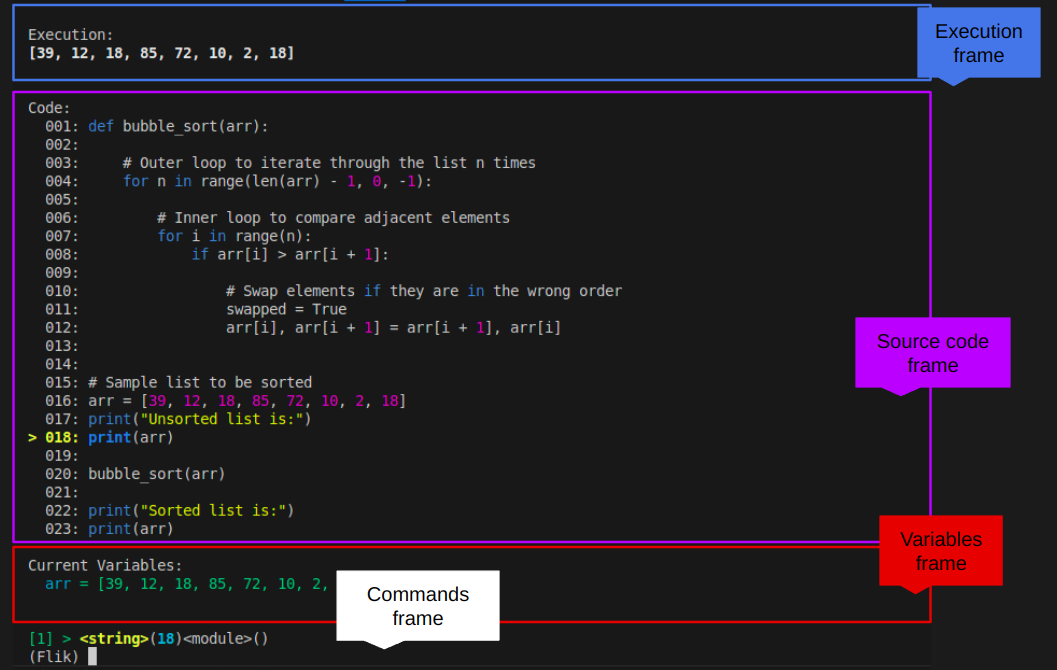
\includegraphics[width=1\textwidth]{figures/flik_interface.png}
    \caption{Debugger tool}
    \label{fig:debuggerf}
\end{figure}

% Add example of use step by step. Explain the videos.
Now, let's use an example to further understand how \flik works. Let's work with 
the usual gridworld example of \ac{RL} programs. The environment is a grid of 
$10 \times 10$ and the agent can move in four directions: up, down, left, and right.
There are two kind of rewards that the agent can get, a positive reward of 1 when 
the agent gets to the goal, and a negative reward of -1 when the agent goes to the 
trap. The agent starts in the blue box shown \fref{fig:gridworld}. Now, in the following
example let's say we define our program properly, but we define the $\epsilon$ value 
so small that the agent will not explore the grid, and will not learn properly. 
This will mean that only the first action taken by the agent will be random and after that
with a major probability it will keep only choosing the same action. We can think about 
the worst case scenario, in which the agent will move right and then in the next step it 
will move left, and it will keep doing this for a long time, with a low probability of 
choosing another action. We can use \flik to debug this problem, we can go step by step
inspecting the variables and the actions taken and we can identify specifically that for 
the first state in each episode the agent is taking the same action. We can then go back and
reproduce this problem as many times as we want, and we can change the value of $\epsilon$
to a higher value, so the agent can explore the grid properly. And finish the execution.
This example is shown in the following video: \url{https://drive.google.com/file/d/1NyipuWsRr6ZrIbtlvU5qyooHS2aVsWXc/view?usp=sharing}.



\endinput

